% Báo cáo BTL KTMT MI4344 — WatchChip. Khung do Claude dựng 27/10/2026 theo bố cục báo cáo Nhóm 3
% (kỳ 2025.1) + mục lục KE-HOACH-LAM-VIEC.md §5. Nội dung/tiêu chí từng mục: report/KHUNG-BAO-CAO.md.
% Biên dịch (XeLaTeX, chạy được cả trên Overleaf):  latexmk -xelatex -outdir=build main.tex
\documentclass[a4paper,12pt,oneside]{report}

\usepackage{fontspec}
% Times, đủ dấu tiếng Việt: Termes có sẵn trên Overleaf/TeX Live; máy Windows không có thì dùng Times New Roman
\IfFontExistsTF{TeX Gyre Termes}{\setmainfont{TeX Gyre Termes}}{\setmainfont{Times New Roman}}
\usepackage{polyglossia}
\setdefaultlanguage{vietnamese}

\usepackage[left=3cm,right=2cm,top=2.5cm,bottom=2.5cm]{geometry}
\usepackage{setspace}\setstretch{1.3}
\setlength{\parindent}{1em}
\setlength{\parskip}{4pt}

\usepackage{graphicx}
\graphicspath{{hinh/}{../}}             % ../ = report/ (h9_dse.png, h_e4_bongma.png)
\usepackage{booktabs,longtable,multirow,array,tabularx}
\usepackage{amsmath}
\usepackage{xcolor}
\usepackage{listings}
\usepackage{tikz}
\usepackage{caption}
\captionsetup{labelsep=colon,labelfont=bf,font=small}
\usepackage{titlesec}
\usepackage{fancyhdr}
\usepackage{tocloft}
\usepackage[hidelinks]{hyperref}

% --- Tên gọi tiếng Việt (gắn vào captionsvietnamese, nếu không polyglossia ghi đè) ---
\gappto\captionsvietnamese{%
  \renewcommand{\contentsname}{MỤC LỤC}%
  \renewcommand{\listfigurename}{DANH MỤC HÌNH VẼ}%
  \renewcommand{\listtablename}{DANH MỤC BẢNG BIỂU}%
  \renewcommand{\bibname}{TÀI LIỆU THAM KHẢO}%
  \renewcommand{\figurename}{Hình}%
  \renewcommand{\tablename}{Bảng}%
  \renewcommand{\chaptername}{CHƯƠNG}%
  \renewcommand{\appendixname}{PHỤ LỤC}}

% --- Tiêu đề chương: "CHƯƠNG 1. GIỚI THIỆU", căn giữa ---
\titleformat{\chapter}[block]{\centering\bfseries\large}{\MakeUppercase{\chaptertitlename}~\thechapter.}{0.4em}{\MakeUppercase}
\titleformat{name=\chapter,numberless}[block]{\centering\bfseries\Large}{}{0pt}{\MakeUppercase}
\titlespacing*{\chapter}{0pt}{0pt}{18pt}
\titleformat{\section}{\bfseries\normalsize}{\thesection}{1em}{}
\titleformat{\subsection}{\bfseries\normalsize}{\thesubsection}{1em}{}
\titleformat{\subsubsection}{\itshape\normalsize}{\thesubsubsection}{1em}{}
\setcounter{secnumdepth}{3}
\setcounter{tocdepth}{2}

% --- Đầu trang: tên chương bên phải + gạch ---
\pagestyle{fancy}
\fancyhf{}
\fancyhead[R]{\small\leftmark}
\fancyfoot[R]{\thepage}
\renewcommand{\chaptermark}[1]{\markboth{\MakeUppercase{\chaptertitlename}~\thechapter.~\MakeUppercase{#1}}{}}
\fancypagestyle{plain}{\fancyhf{}\fancyfoot[R]{\thepage}\renewcommand{\headrulewidth}{0pt}}

% --- Mục lục: tên chương in đậm ---
\renewcommand{\cftchapfont}{\bfseries}
\renewcommand{\cfttoctitlefont}{\hfill\bfseries\large}\renewcommand{\cftaftertoctitle}{\hfill}
\renewcommand{\cftloftitlefont}{\hfill\bfseries\large}\renewcommand{\cftafterloftitle}{\hfill}
\renewcommand{\cftlottitlefont}{\hfill\bfseries\large}\renewcommand{\cftafterlottitle}{\hfill}
\setlength{\cftbeforetoctitleskip}{0pt}\setlength{\cftbeforeloftitleskip}{0pt}\setlength{\cftbeforelottitleskip}{0pt}
\renewcommand{\cftfigpresnum}{Hình }
\renewcommand{\cfttabpresnum}{Bảng }
\setlength{\cftfignumwidth}{5em}
\setlength{\cfttabnumwidth}{5em}

% --- Code Verilog / MIPS ---
\lstset{basicstyle=\ttfamily\footnotesize,frame=single,numbers=left,numberstyle=\tiny,
        breaklines=true,columns=fullflexible,keepspaces=true}

% --- Macro cho khung: xóa hết trước khi nộp (grep TODO) ---
\newcommand{\TODO}[1]{\par\noindent\colorbox{yellow!30}{\parbox{\dimexpr\linewidth-2\fboxsep}{\small\textbf{TODO:} #1}}\par}
\newcommand{\TODOmssv}{\textit{MSSV}}
% Hình chưa có: \hinhtrong{chú thích}{chủ}{gợi ý}
\newcommand{\hinhtrong}[3]{\begin{figure}[htbp]\centering
  \fbox{\parbox[c][4cm][c]{0.8\linewidth}{\centering\small\textit{Chưa có hình — chủ: #2}\\#3}}
  \caption{#1}\end{figure}}

\begin{document}

% Bìa: khung đôi đỏ/đen như báo cáo Nhóm 3. Logo: đặt hinh/logo-hust.png, hinh/logo-fami.png
\begin{titlepage}
\begin{tikzpicture}[remember picture,overlay]
  \draw[line width=3pt,red!70!black] ([xshift=1.5cm,yshift=-1.5cm]current page.north west) rectangle ([xshift=-1.5cm,yshift=1.5cm]current page.south east);
  \draw[line width=0.6pt] ([xshift=1.2cm,yshift=-1.2cm]current page.north west) rectangle ([xshift=-1.2cm,yshift=1.2cm]current page.south east);
\end{tikzpicture}
\centering\setstretch{1.15}
{\bfseries\large ĐẠI HỌC BÁCH KHOA HÀ NỘI\\ KHOA TOÁN -- TIN\par}
\vspace{1.2cm}
\IfFileExists{hinh/logo-hust.png}{\includegraphics[height=3.5cm]{logo-hust}}{\fbox{\parbox[c][3.5cm][c]{3cm}{\centering logo HUST}}}
\hspace{1.5cm}
\IfFileExists{hinh/logo-fami.png}{\includegraphics[height=3.5cm]{logo-fami}}{\fbox{\parbox[c][3.5cm][c]{3cm}{\centering logo FaMI}}}
\par\vspace{1.2cm}
{\bfseries\fontsize{26}{32}\selectfont BÁO CÁO\\[4pt] KIẾN TRÚC MÁY TÍNH\par}
\vspace{0.8cm}
{\bfseries\Large Chủ đề: Thiết kế SoC đồng hồ điện tử WatchChip\\ trên CPU MIPS tự thiết kế (đơn chu kỳ và pipeline)\par}
\vspace{1.2cm}
\begin{tabular}{r l l}
Sinh viên: & \textbf{Đoàn Danh Long} & \TODOmssv \\
           & \textbf{TV1 — chưa điền} & \TODOmssv \\
           & \textbf{TV2 — chưa điền} & \TODOmssv \\
           & \textbf{TV3 — chưa điền} & \TODOmssv \\
           & \textbf{TV4 — chưa điền} & \TODOmssv \\
           & \textbf{TV5 — chưa điền} & \TODOmssv \\
Lớp: & \textbf{chưa điền} & \\
Giảng viên giảng dạy: & \textbf{chưa điền} & \\
\end{tabular}
\vfill
{\bfseries\large HÀ NỘI, 12/2026\par}
\vspace{1cm}
\end{titlepage}


\pagenumbering{roman}
\tableofcontents
\clearpage\listoffigures
\clearpage\listoftables

\chapter*{Lời giới thiệu}
\addcontentsline{toc}{chapter}{LỜI GIỚI THIỆU}
\markboth{LỜI GIỚI THIỆU}{}

\TODO{Long viết (1 trang). Nêu: bài toán (đồng hồ chuẩn ms), đề tài, phạm vi \textbf{chỉ mô phỏng} (không board, không Fmax), lời cảm ơn giảng viên. Không hứa điều báo cáo không chứng minh.}

\begin{flushright}
\textit{Hà Nội, ngày \ldots{} tháng 12 năm 2026}\\
\textbf{Nhóm \ldots}
\end{flushright}


\cleardoublepage
\pagenumbering{arabic}
\chapter{GIỚI THIỆU}

\section{Bài toán}\label{sec:bai-toan}
Đề tài thiết kế \textbf{WatchChip}: con chip của một chiếc đồng hồ điện tử kiểu Casio F-91W, viết bằng Verilog. Chip có CPU MIPS32 tự viết, bộ đếm thời gian, hiển thị LED 7 đoạn và VGA, còi, UART và ngắt. CPU có hai bản: \textbf{G1} chạy đơn chu kỳ, \textbf{G2} chạy đường ống 5 tầng. Cả hai chạy cùng một tập 28 lệnh và cùng một firmware.

Đồng hồ có năm chế độ: xem giờ, chỉnh giờ, bấm giờ, hẹn giờ (đếm xuống 0 rồi đếm tiếp sang số âm) và báo thức. Giờ có thể đồng bộ với máy tính qua UART.

Câu hỏi xuyên suốt của đồ án là: \emph{muốn đồng hồ chuẩn tới 1 ms thì phần nào phải là phần cứng?} Phép tính mở đầu rất ngắn. Để sai không quá 1 ms sau 1 giờ (3600 s), tần số phải sai không quá $1\,\text{ms} / 3600\,\text{s} = 0{,}28$ ppm. Một thạch anh thông thường sai cỡ $\pm 50$ ppm (giả định, chưa kiểm datasheet), tức lệch $50 \times 10^{-6} \times 3600 = 0{,}18$ s mỗi giờ. Vì vậy chip cần hiệu chỉnh tần số theo giờ chuẩn từ máy tính (thanh ghi 	exttt{CAL}) và cần bộ đếm phần cứng. Câu trả lời bằng số đo nằm ở mục~\ref{sec:thi-nghiem}.

\paragraph{Phạm vi.} Đề tài chỉ chạy trong mô phỏng, không nạp lên board. Để mô phỏng nhanh, 1 ms của chip được rút thành $G_N = 50$ nhịp xung hệ thống thay vì 50\,000. Mục~\ref{sec:cong-cu} nói rõ hệ quả của hai điều này.

\section{Cơ sở lý thuyết: kiến trúc tập lệnh MIPS}\label{sec:mips}
\subsection{Tổng quan MIPS ISA}
Kiến trúc tập lệnh (ISA) là hợp đồng giữa phần mềm và phần cứng: lệnh nào có, mã hóa ra sao, mỗi lệnh làm gì. MIPS là ISA kiểu RISC: lệnh dài cố định 32 bit, chỉ \texttt{lw} và \texttt{sw} mới đụng bộ nhớ, mọi phép tính khác lấy toán hạng từ thanh ghi.

WatchChip dùng một tập con gồm 28 lệnh của MIPS32, cộng một lệnh riêng \texttt{bcd} (mục~\ref{sec:lenh}). Ba điểm khác với MIPS đầy đủ cần nhớ:
\begin{itemize}
  \item không có \emph{delay slot}: lệnh ngay sau nhánh hoặc nhảy chỉ chạy khi nhánh không nhảy;
  \item không có ngoại lệ tràn số, lệnh lạ hay địa chỉ sai; nguồn duy nhất vào vector \texttt{0x180} là ngắt;
  \item bộ nhớ kiểu Harvard: bộ nhớ lệnh (IMEM) và bộ nhớ dữ liệu (DMEM) tách riêng.
\end{itemize}

\subsection{Tập thanh ghi}
Có 32 thanh ghi 32 bit \texttt{\$0}--\texttt{\$31}; \texttt{\$0} luôn đọc ra 0 và ghi vào bị bỏ. \texttt{jal} ghi địa chỉ quay về vào \texttt{\$31} (\texttt{\$ra}). Hai thanh ghi \texttt{HI} và \texttt{LO} giữ kết quả của \texttt{div}. Ba thanh ghi của bộ đồng xử lý CP0 dùng cho ngắt: \texttt{\$12} Status, \texttt{\$13} Cause, \texttt{\$14} EPC (mục~\ref{sec:ngat-lt}). Bộ đếm chương trình PC dài 32 bit, địa chỉ tính theo byte, lệnh luôn căn 4.

\subsection{Định dạng lệnh và 28 lệnh được hỗ trợ}\label{sec:lenh}
Mọi lệnh dài 32 bit và thuộc một trong ba khuôn chính R, I, J. Hai nhóm \texttt{SPECIAL2} và \texttt{COP0} dùng lại khuôn R với vài trường được gán nghĩa riêng.

\begin{table}[htbp]
\centering\small
\begin{tabular}{@{}lllllll@{}}
\toprule
Khuôn & {[}31:26{]} & {[}25:21{]} & {[}20:16{]} & {[}15:11{]} & {[}10:6{]} & {[}5:0{]} \\
\midrule
R        & \texttt{op} = 0 & \texttt{rs} & \texttt{rt} & \texttt{rd} & \texttt{shamt} & \texttt{funct} \\
I        & \texttt{op}     & \texttt{rs} & \texttt{rt} & \multicolumn{3}{l}{\texttt{imm} (16 bit)} \\
J        & \texttt{op}     & \multicolumn{5}{l}{\texttt{target} (26 bit)} \\
SPECIAL2 & \texttt{0x1C}   & \texttt{rs} & \texttt{rt} & \texttt{rd} & 0 & \texttt{funct} \\
COP0     & \texttt{0x10}   & \texttt{sub} & \texttt{rt} & \texttt{rd} & 0 & 0 hoặc \texttt{0x18} \\
\bottomrule
\end{tabular}
\caption{Các khuôn lệnh của WatchChip.}\label{tab:khuon}
\end{table}

Ký hiệu: $\mathtt{R[x]}$ là thanh ghi, $\mathtt{M[a]}$ là một word của bộ nhớ, $\mathtt{s(x)}$ hiểu số có dấu, $\mathtt{u(x)}$ hiểu số không dấu. $\mathtt{SE(imm)}$ là mở rộng dấu 16 lên 32 bit, $\mathtt{ZE(imm)}$ là mở rộng bằng 0. Đích nhánh là $\mathtt{PC + 4 + (SE(imm) \ll 2)}$; đích \texttt{j} và \texttt{jal} là 4 bit cao của $\mathtt{PC + 4}$ ghép với \texttt{target} và hai bit 0. Phép cộng và trừ lấy 32 bit thấp, không bẫy tràn. Trong \texttt{sub} của COP0, \texttt{0x00} là \texttt{mfc0}, \texttt{0x04} là \texttt{mtc0}, \texttt{0x10} là \texttt{eret}.

Tập lệnh gồm 12 lệnh khuôn R, 9 lệnh khuôn I, 2 lệnh khuôn J, 2 lệnh \texttt{SPECIAL2} (\texttt{mul}, \texttt{bcd}) và 3 lệnh COP0, tổng 28. Bảng~\ref{tab:isa28} liệt kê từng lệnh.

{\small
\begin{longtable}{@{}r p{3.6cm} l p{6.1cm}@{}}
\caption{28 lệnh của WatchChip: mã hóa và ý nghĩa.}\label{tab:isa28}\\
\toprule
\# & Lệnh & op / funct & Ý nghĩa \\
\midrule
\endfirsthead
\toprule
\# & Lệnh & op / funct & Ý nghĩa \\
\midrule
\endhead
\bottomrule
\endfoot
1 & \texttt{addu rd,rs,rt} & 00/0x21 & \texttt{R[rd] = R[rs] + R[rt]} \\
2 & \texttt{subu rd,rs,rt} & 00/0x23 & \texttt{R[rd] = R[rs] $-$ R[rt]} \\
3 & \texttt{and rd,rs,rt} & 00/0x24 & \texttt{R[rd] = R[rs] \& R[rt]} \\
4 & \texttt{or rd,rs,rt} & 00/0x25 & \texttt{R[rd] = R[rs] \textbar{} R[rt]} \\
5 & \texttt{xor rd,rs,rt} & 00/0x26 & \texttt{R[rd] = R[rs] \^{} R[rt]} \\
6 & \texttt{slt rd,rs,rt} & 00/0x2A & \texttt{R[rd] = s(R[rs]) < s(R[rt]) ? 1 : 0} \\
7 & \texttt{sll rd,rt,sa} & 00/0x00 & \texttt{R[rd] = R[rt] {<}{<} sa} (\texttt{sll \$0,\$0,0} = \texttt{nop} = 0x00000000) \\
8 & \texttt{sra rd,rt,sa} & 00/0x03 & \texttt{R[rd] = s(R[rt]) {>}{>} sa} (dịch số học, chép bit dấu) \\
9 & \texttt{jr rs} & 00/0x08 & \texttt{PC = R[rs]} (2 bit thấp bị bỏ) \\
10 & \texttt{div rs,rt} & 00/0x1A & Chia có dấu: \texttt{LO} = thương làm tròn về 0, \texttt{HI} = dư (cùng dấu với số bị chia). Chạy 33 chu kỳ CPU (một chu kỳ start, 32 bước chia). \\
11 & \texttt{mfhi rd} & 00/0x10 & \texttt{R[rd] = HI} \\
12 & \texttt{mflo rd} & 00/0x12 & \texttt{R[rd] = LO} \\
13 & \texttt{addiu rt,rs,imm} & 0x09 & \texttt{R[rt] = R[rs] + SE(imm)} \\
14 & \texttt{slti rt,rs,imm} & 0x0A & \texttt{R[rt] = s(R[rs]) < s(SE(imm)) ? 1 : 0} \\
15 & \texttt{andi rt,rs,imm} & 0x0C & \texttt{R[rt] = R[rs] \& ZE(imm)} \\
16 & \texttt{ori rt,rs,imm} & 0x0D & \texttt{R[rt] = R[rs] \textbar{} ZE(imm)} \\
17 & \texttt{lui rt,imm} & 0x0F & \texttt{R[rt] = imm {<}{<} 16} \\
18 & \texttt{lw rt,imm(rs)} & 0x23 & \texttt{R[rt] = M[(R[rs] + SE(imm)) \& \~{}3]} \\
19 & \texttt{sw rt,imm(rs)} & 0x2B & \texttt{M[(R[rs] + SE(imm)) \& \~{}3] = R[rt]} \\
20 & \texttt{beq rs,rt,L} & 0x04 & Nếu \texttt{R[rs] == R[rt]} thì \texttt{PC = PC + 4 + (SE(imm) {<}{<} 2)}. \\
21 & \texttt{bne rs,rt,L} & 0x05 & Nếu \texttt{R[rs] != R[rt]} thì \texttt{PC = PC + 4 + (SE(imm) {<}{<} 2)}. \\
22 & \texttt{j L} & 0x02 & Nhảy tới địa chỉ ghép từ \texttt{target} (xem trên). \\
23 & \texttt{jal L} & 0x03 & \texttt{R[31] = PC + 4}, rồi nhảy như \texttt{j}. \\
24 & \texttt{mul rd,rs,rt} & 0x1C/0x02 & \texttt{R[rd]} = 32 bit thấp của tích có dấu \texttt{s(R[rs])} $\times$ \texttt{s(R[rt])}. \texttt{HI}, \texttt{LO} không đổi. \\
25 & \texttt{bcd rd,rs} & 0x1C/0x10 & Nếu \texttt{u(R[rs])} $\le$ 99\,999\,999 thì \texttt{R[rd]} gồm 8 chữ số thập phân, mỗi chữ số 4 bit, hàng đơn vị ở bit [3:0]; ngược lại \texttt{R[rd] = 0xFFFFFFFF}. \\
26 & \texttt{mfc0 rt,rd} & 0x10/rs = 0x00 & \texttt{R[rt] = CP0[rd]} \\
27 & \texttt{mtc0 rt,rd} & 0x10/rs = 0x04 & \texttt{CP0[rd] = R[rt]} (chỉ ghi các bit ghi được). \\
28 & \texttt{eret} & 0x42000018 & \texttt{PC = EPC}, \texttt{Status.EXL = 0} \\
\end{longtable}
}

\section{Cơ sở thiết kế}\label{sec:co-so-tk}
\subsection{CPU đơn chu kỳ}
CPU đơn chu kỳ làm xong một lệnh trong một chu kỳ: lấy lệnh, giải mã, đọc thanh ghi, tính, truy cập bộ nhớ, ghi kết quả. CPI (số chu kỳ trên một lệnh) bằng 1. Đổi lại, chu kỳ xung phải dài bằng đường đi chậm nhất, thường là của \texttt{lw}, nên mọi lệnh đều phải chờ theo nó. Thiết kế này dễ kiểm nhất và là cơ sở để so sánh. WatchChip hiện thực nó thành G1, với một sửa đổi cho bộ nhớ trong FPGA (mục~\ref{sec:g1}).

\subsection{Kỹ thuật đường ống (pipelining)}
Đường ống chia lệnh thành các tầng và cho nhiều lệnh chạy chồng nhau, mỗi lệnh ở một tầng khác nhau. Năm tầng cổ điển là IF (lấy lệnh), ID (giải mã, đọc thanh ghi), EX (tính), MEM (truy cập bộ nhớ) và WB (ghi thanh ghi). Giữa hai tầng có một thanh ghi tầng giữ kết quả dở dang. Khi đầy ống, mỗi chu kỳ xong một lệnh, và chu kỳ xung chỉ cần dài bằng tầng chậm nhất, ngắn hơn nhiều so với đơn chu kỳ. WatchChip hiện thực nó thành G2.

\subsection{Các loại xung đột và kỹ thuật xử lý}
Xung đột (hazard) là tình huống lệnh kế tiếp không thể chạy ngay ở chu kỳ kế. Có ba loại:
\begin{itemize}
  \item \textbf{Xung đột cấu trúc}: hai lệnh cần cùng một tài nguyên phần cứng trong cùng chu kỳ, ví dụ cùng đọc một bộ nhớ để lấy lệnh và để lấy dữ liệu. Tách IMEM và DMEM (kiểu Harvard) loại bỏ trường hợp này.
  \item \textbf{Xung đột dữ liệu}: lệnh sau cần kết quả lệnh trước chưa kịp ghi (RAW, đọc sau ghi). Kỹ thuật xử lý là \emph{forwarding}: đưa kết quả thẳng từ đầu ra một tầng về đầu vào ALU, không đợi ghi vào thanh ghi. Riêng \texttt{lw} có dữ liệu muộn hơn: lệnh dùng ngay kết quả của nó phải \emph{đứng} (stall) một chu kỳ. Đó là xung đột load-use.
  \item \textbf{Xung đột điều khiển}: chưa biết nhánh có nhảy hay không thì chưa biết lệnh kế là lệnh nào. Cách đơn giản nhất là dự đoán không nhảy; nếu đoán sai thì hủy (flush) các lệnh đã lấy nhầm.
\end{itemize}
Chương~\ref{chap:thiet-ke} nói từng loại được xử lý thế nào trong G2.

\subsection{Ngắt và CP0}\label{sec:ngat-lt}
Ngắt cho ngoại vi (ở đây là nút bấm, UART) chen vào chương trình đang chạy mà không cần CPU hỏi liên tục. Khi nhận ngắt, CPU lưu địa chỉ lệnh cần quay về vào \texttt{EPC}, bật cờ \texttt{EXL} để chặn ngắt lồng, rồi nhảy tới địa chỉ cố định \texttt{0x180}. Trình xử lý kết thúc bằng \texttt{eret}: PC lấy lại từ \texttt{EPC} và \texttt{EXL} xóa về 0. Các thanh ghi \texttt{Status}, \texttt{Cause}, \texttt{EPC} nằm trong CP0 và đọc, ghi bằng \texttt{mfc0}, \texttt{mtc0}. Ngắt \emph{chính xác} nghĩa là lệnh nào đã qua một điểm nhất định thì chạy trọn, lệnh chưa qua thì bị hủy và chạy lại sau \texttt{eret}; điều này quan trọng với đường ống, nơi nhiều lệnh dở dang cùng lúc.

\TODO{Long. Chèn tối đa 3 hình từ sách Patterson \& Hennessy cho mục 1.3 (đường dữ liệu đơn chu kỳ, đường ống 5 tầng, forwarding), mỗi hình ghi ``nguồn: P\&H Fig x.y''. Báo cáo chỉ được dùng hình sách ở chương 1.}

\chapter{PHƯƠNG PHÁP LUẬN VÀ THIẾT KẾ}

\section{Công cụ và cấu trúc mã nguồn}
\TODO{TV2. Verilog; iverilog + ModelSim (mô phỏng), Yosys (tổng hợp); Python (\texttt{asm.py}, \texttt{iss.py}, \texttt{cmp\_trace.py}); cây thư mục (\texttt{KE-HOACH} §6); testbench. Ghi rõ: không có Vivado/Quartus nên không có Fmax.}

\section{Tổng thể SoC}
\hinhtrong{Sơ đồ tổng thể SoC WatchChip (H1)}{TV3}{khối trên hình = module trong \texttt{soc\_top.v}}
\TODO{TV3. Thông số (IMEM/DMEM, xung nhịp mô phỏng), giao diện vào/ra.}

\section{Bộ điều khiển hiển thị}
\TODO{TV4. Display RAM, ROM ký tự, quét 7 đoạn (khoảng tắt \texttt{G\_BLANK}, bản sửa 27/10), VGA đuổi tia. Nháp: \texttt{report/2.3-vga.md}. Khớp \texttt{docs/display-spec.md}.}
\hinhtrong{Bộ điều khiển hiển thị và giản đồ thời gian quét có khoảng tắt (H7)}{TV4}{khớp \texttt{display-spec.md} §4}

\section{Timebase, hiệu chỉnh CAL và các bộ định thời}
\TODO{TV5. Timebase + \texttt{CAL}, RTC, stopwatch có capture, TIMER đếm ngược, alarm, nút. Phần thí nghiệm E1$'$/E2$'$ đặt ở mục~\ref{sec:thi-nghiem}.}
\hinhtrong{Timebase và các bộ định thời, có đường capture (H5)}{TV5}{}

\section{Bus, MMIO, bộ điều khiển ngắt, UART, bộ tạo âm}
\TODO{TV4/TV3. Nháp UART + ngắt UART\_RX: \texttt{report/2.5-uart-sync-ngat.md}. Bảng địa chỉ khớp \texttt{docs/mmio-map.md}.}
\hinhtrong{Bản đồ địa chỉ MMIO (H6)}{TV4}{khớp \texttt{mmio-map.md}}

\section{CPU G1: đơn chu kỳ}
\subsection{Datapath}
\hinhtrong{Datapath CPU G1 (H2)}{TV1}{mỗi tên tín hiệu có trong \texttt{cpu\_g1.v}}
\subsection{Khối điều khiển và bảng chân lý}
\TODO{TV3. Bảng chân lý cho \textbf{cả 28 lệnh}, khớp \texttt{docs/control-table.md}.}
\subsection{CP0 và ngắt}
\subsection{Vì sao chọn: G1 hai pha (BRAM sườn xuống) hay LUT-RAM}

\section{CPU G2: pipeline 5 tầng}
\hinhtrong{Datapath CPU G2 đầy đủ (H3)}{TV3}{}
\subsection{Thanh ghi đường ống}
\TODO{TV3. Bảng trường + độ rộng từng thanh ghi tầng, khớp \texttt{cpu\_pipe.v}.}

\section{Xử lý xung đột}
\TODO{TV2. Mỗi loại đi đủ 5 bước: định nghĩa $\rightarrow$ biểu thức điều kiện $\rightarrow$ khối phần cứng $\rightarrow$ đoạn code $\rightarrow$ \textbf{bảng diễn biến theo chu kỳ}. Bảng chu kỳ khớp \texttt{docs/pipeline-policy.md} §7.}
\hinhtrong{Khối forwarding và hazard unit (H4)}{TV2}{}
\subsection{RAW ở EX và ở MEM: forwarding}
\subsection{Load-use: stall}
\subsection{Rẽ nhánh: quyết định ở EX, flush}
\subsection{\texttt{busy} freeze khi \texttt{div}/\texttt{bcd}}
\subsection{\texttt{mtc0} $\rightarrow$ \texttt{mfc0}}
\subsection{\texttt{eret} và vào/ra ngắt}
\subsection{Vì sao chọn}
\TODO{So sánh $\geq 2$ phương án rồi chốt: nhánh ở EX hay ID (bảng T4), bộ đếm nhị phân hay BCD, \texttt{bcd} tổ hợp hay tuần tự, polling hay ngắt, VGA đuổi tia hay framebuffer.}

\section{ALU, nhân, chia và lệnh \texttt{bcd}}
\TODO{TV1. ALU, \texttt{muldiv}, \texttt{bcd\_unit} hai bản.}

\section{Firmware}
\TODO{TV2/TV5. 5 chế độ, \texttt{fmt}, đồng bộ giờ qua UART + \texttt{CAL} (bộ đệm đôi, 27/10). Một phần đã có trong \texttt{report/2.5-uart-sync-ngat.md}.}

\section{Hiện thực các module chính}
\TODO{Mỗi chủ gói trích 1 đoạn code ngắn có chú thích, đúng file hiện tại (\texttt{\textbackslash lstinputlisting} với \texttt{firstline/lastline}).}

\chapter{KIỂM THỬ VÀ KẾT QUẢ}

\section{Chiến lược kiểm thử}
\TODO{TV2/TV4. Unit $\rightarrow$ co-sim ISS $\rightarrow$ bộ test hazard $\rightarrow$ \texttt{system\_tb} (G1 và G2, có/không ngắt) $\rightarrow$ màn hình ảo; kiểm thử đột biến. Số kiểm lấy từ hồi quy mới nhất trong \texttt{evidence/}. Nháp màn ảo: \texttt{report/3.1-man-ao.md}.}

\section{Trace và dạng sóng}
\hinhtrong{Dạng sóng: load-use bubble, flush nhánh, \texttt{busy} freeze, vào/ra ngắt (H8)}{TV3}{4 ảnh, chú thích chu kỳ khớp \texttt{pipeline-policy.md} §7}

\section{Hiệu năng G1 và G2: CPI tách theo nguyên nhân}
\TODO{TV2/TV3. Số đếm bằng \texttt{tools/cpi.py}, không ``$\approx$''. Nháp: \texttt{report/3.3-cpi.md}.}

\section{Khảo sát thiết kế (DSE) và tài nguyên}
\TODO{TV1. Nháp: \texttt{report/3.4-dse.md}; còn thiếu phần tài nguyên (plan §8.2).}
\begin{figure}[htbp]\centering
  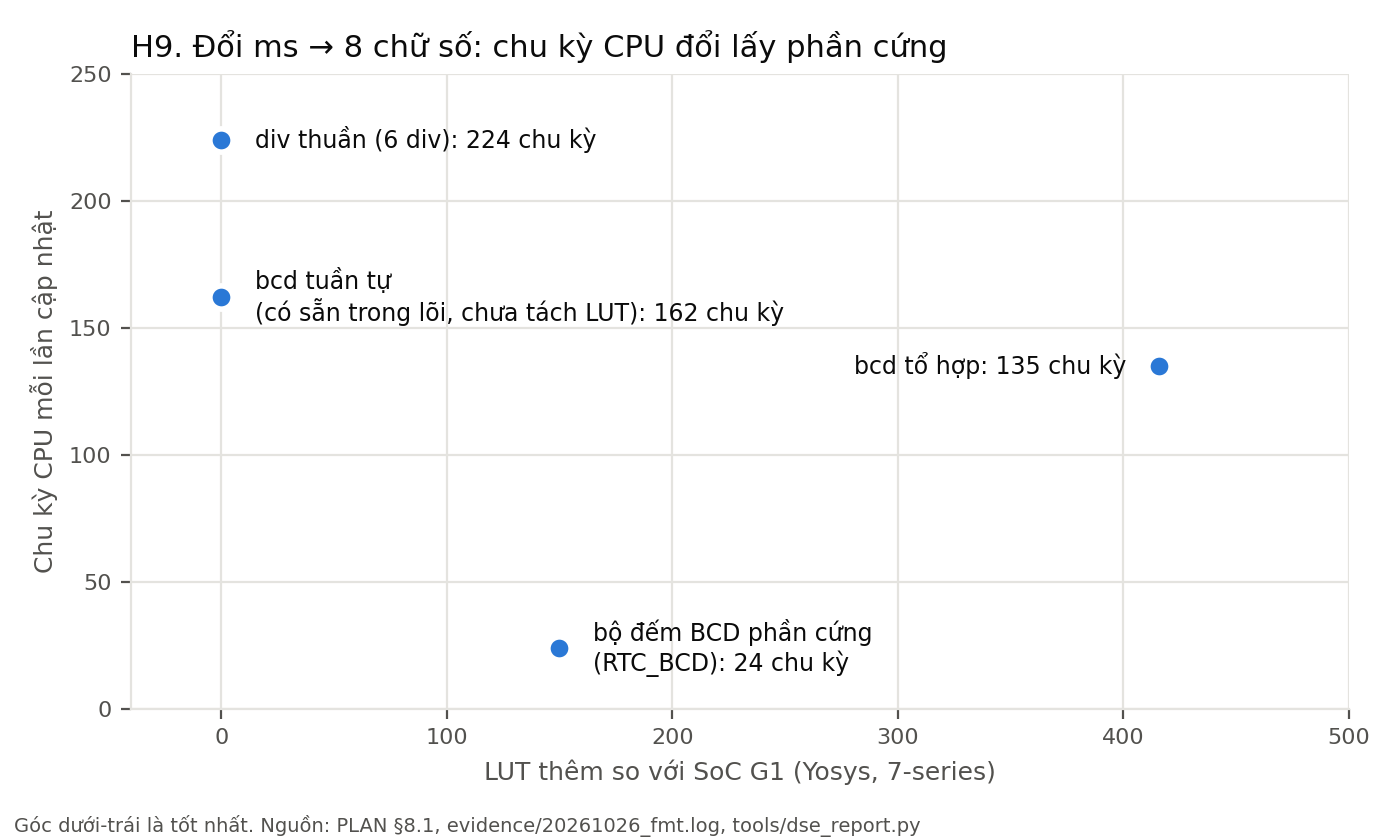
\includegraphics[width=0.85\linewidth]{h9_dse}
  \caption{Chi phí đổi ms sang chữ số (H9)}
\end{figure}

\section{Thí nghiệm E1$'$--E4$'$}\label{sec:thi-nghiem}
\TODO{Mỗi thí nghiệm: câu hỏi $\rightarrow$ cách đo $\rightarrow$ bảng/hình $\rightarrow$ kết luận + phạm vi đúng. Trả lời câu hỏi ``chuẩn ms'' của chương 1.}
\subsection{E1$'$, E2$'$: hiệu chỉnh CAL}
\TODO{TV5. Nháp: \texttt{report/2.4-cal-thi-nghiem.md}.}
\subsection{E3: polling, ngắt và capture}
\TODO{TV3 + TV2. Nháp: \texttt{report/2.5-e3-thi-nghiem.md}.}
\subsection{E4$'$: bóng ma khi quét 7 đoạn}
\TODO{TV4. Nháp: \texttt{report/2.3-bongma-e4.md}. Kèm H10 (màn hình ảo).}
\begin{figure}[htbp]\centering
  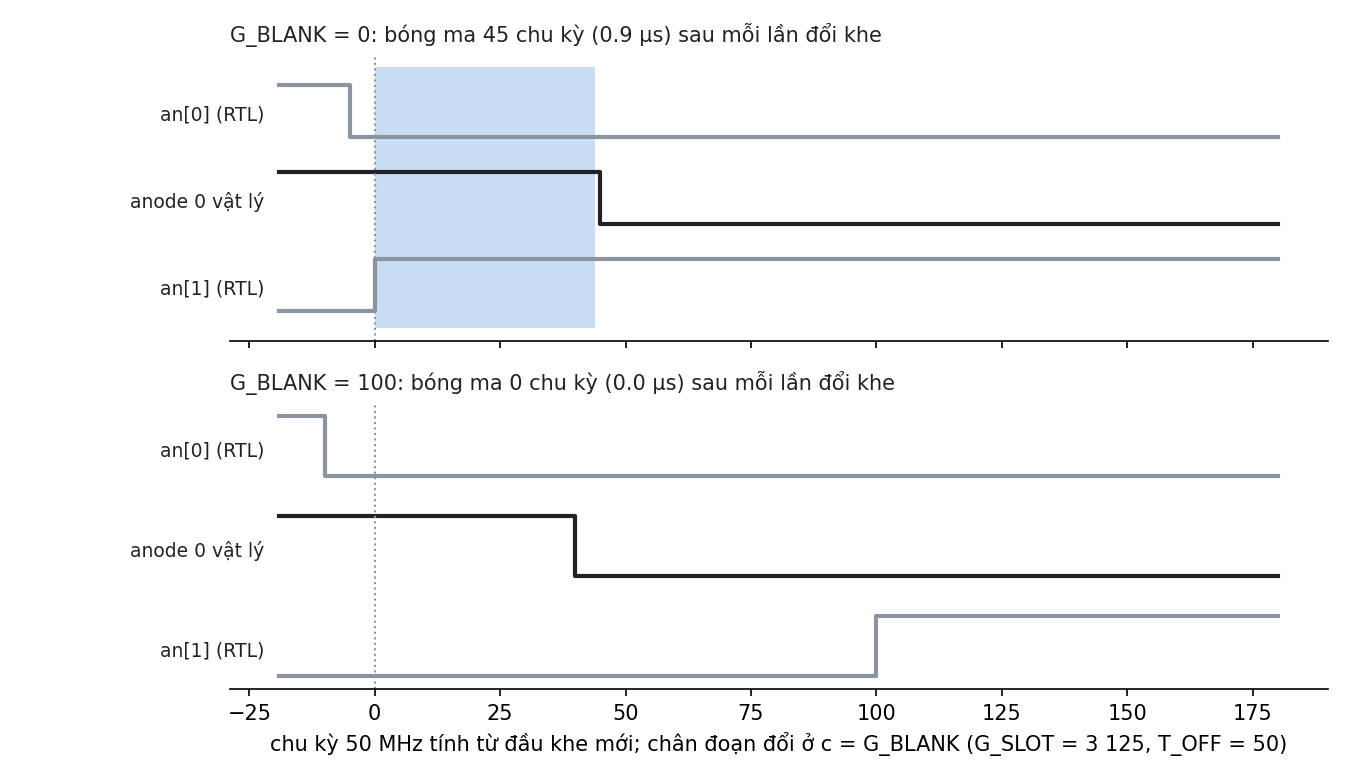
\includegraphics[width=0.85\linewidth]{h_e4_bongma}
  \caption{Bóng ma theo thời gian tắt của chân đoạn, ở 3 giá trị \texttt{G\_SLOT}}
\end{figure}

\section{Tổng kết: đạt và chưa đạt}
\TODO{TV2. Nháp: \texttt{report/3.6-bang-dat.md}. Mỗi dòng trỏ về 1 file \texttt{evidence/}; người viết tự chạy lại rồi mới tick.}

\chapter{KẾT LUẬN VÀ HƯỚNG PHÁT TRIỂN}

\section{Kết quả đạt được}
\TODO{Long. Tóm tắt có số, mỗi số trỏ về mục chương 3.}

\section{Hạn chế}
\TODO{Long. Lấy đúng cột CHƯA ĐẠT của bảng tổng kết, có số: chỉ mô phỏng, không Fmax, $\geq 3$ câu UART liền nhau bị chụp giờ trễ, race PENDING chưa test tất định, \ldots}

\section{Hướng phát triển}
\TODO{Long. Nạp board + đo thật; \texttt{sync\_host.py} phía PC; hàng đợi vòng cho UART; Fmax khi có công cụ FPGA.}


\appendix
\chapter{PHÂN CÔNG CÔNG VIỆC}
\begin{table}[htbp]\centering
\caption{Phân công nhiệm vụ và đóng góp}
\begin{tabularx}{\linewidth}{|c|l|c|X|c|X|}
\hline
\textbf{STT} & \textbf{Họ và tên} & \textbf{MSSV} & \textbf{Gói phụ trách} & \textbf{\%} & \textbf{Bằng chứng} \\ \hline
1 & Đoàn Danh Long & & biên tập, \ldots & & \\ \hline
2 & TV1 & & ALU \& số học & & \\ \hline
3 & TV2 & & công cụ \& hazard & & \\ \hline
4 & TV3 & & CPU \& chip & & \\ \hline
5 & TV4 & & hiển thị \& âm thanh & & \\ \hline
6 & TV5 & & định thời ms & & \\ \hline
\end{tabularx}
\end{table}
\TODO{Long. Đóng góp ghi \% (không ghi thang 1--5 như Nhóm 3), kèm bằng chứng (\texttt{hop-tuan.md}, kết quả cổng). Chốt cách khai phần AI viết (\texttt{KE-HOACH} §4b).}

\chapter{KẾ HOẠCH VÀ TIẾN ĐỘ}
\TODO{Long. Bảng kế hoạch (\texttt{docs/goi-viec.md}) đặt cạnh thực tế (\texttt{docs/hop-tuan.md} + worklog), theo tuần.}

\chapter{HƯỚNG DẪN CHẠY LẠI}
\TODO{TV2. Người khác chạy được trên máy họ. Tối thiểu:}
\begin{lstlisting}[language=bash,numbers=none]
source tools/env.sh
bash tools/run_unit.sh          # full regression
python tools/cosim_iss.py --g2 --rand 0
\end{lstlisting}

\chapter{TRÍCH TRACE VÀ LOG}
\TODO{TV2. Trích ngắn từ \texttt{evidence/}, ghi tên file gốc.}


\begin{thebibliography}{9}
\addcontentsline{toc}{chapter}{TÀI LIỆU THAM KHẢO}
\bibitem{ph} D.~A. Patterson, J.~L. Hennessy. \textit{Computer Organization and Design: The Hardware/Software Interface}, MIPS Edition. Morgan Kaufmann.
\bibitem{mips2} MIPS Technologies. \textit{MIPS32 Architecture for Programmers, Volume II: The MIPS32 Instruction Set}.
\bibitem{mips3} MIPS Technologies. \textit{MIPS32 Architecture for Programmers, Volume III: The MIPS32 Privileged Resource Architecture}.
\bibitem{casio} Casio. \textit{Operation Guide, Module 593}.
\bibitem{ds3231} Maxim Integrated. \textit{DS3231 Extremely Accurate I2C-Integrated RTC/TCXO/Crystal}, datasheet.
\bibitem{stm32} STMicroelectronics. \textit{Reference manual RM0008: STM32F10x}.
\end{thebibliography}
\TODO{Kiểm lại ấn bản/năm từng mục trước khi nộp.}


\end{document}
